% !TEX root = Master.tex

\begin{table}[H]
\setlength\arrayrulewidth{1pt}  
\centering
\begin{adjustbox}{max width=\textwidth}
\begin{tabular}{|c|c|c|}
\hline
\rowcolor{Gray}
\textbf{Variable}    & \textbf{Data Type} & \textbf{Dataset}       \\ \hline
Diameter {[}cm{]}    & Continuous         & Inventory              \\ \hline
Crown Area {[}cm²{]} & Continuous         & LiDAR                  \\ \hline
Height {[}cm{]}      & Continuous         & LiDAR                  \\ \hline
Species (Art\_ grp)  & Factor             & LiDAR (Neural Networks) \\ \hline
\end{tabular}
\end{adjustbox}

\caption{Variables used in the study and their sources}
\label{tab:variables}
\end{table}

First the general properties of the inventory data of 2018 are examined to obtain a first intuition of dependencies
and structures for further analysis. As discussed in Section \ref{Methodology}, the diameter is predicted based on some
variables. Previous research proposed to create models individually for each tree species, using height
measurements, the crown area \& the crown area of larger trees [6].\\

Figure \ref{fig:boxplots Overview} indicates that this proposition is also valid for the measured trees in Gartow, as the boxplots of the
diameter and height differ per species. Similar patterns are seen for height and diameter,
indicating high correlation.

\begin{figure}[H]
\centering
  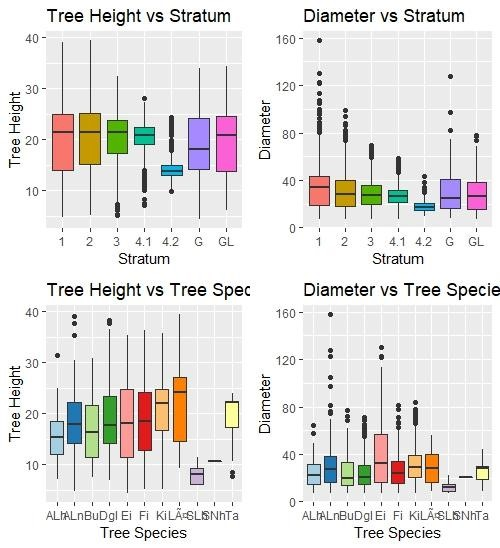
\includegraphics[scale = 0.8]{boxplots_overview.jpg}
  \caption{Boxplots based on Stratum (upper) and Tree Species (lower). Same patterns show potential correlation in height and diameter.}
  \label{fig:boxplots Overview}
\end{figure}

Figure \ref{fig:diameter vs height} underlines this expected height correlation. A strong non-linear relationship is observed. This almost
exponential curve can be explained by the natural growth of a tree. Once a tree species reaches its maximum
height, only the diameter continues to grow up to a natural limit. The effect of tree specific is well observable
comparing oaks (Ei) and pines (Ki). They are well separated between 20 and 30 meters of height.

\begin{figure}[H]
\centering
  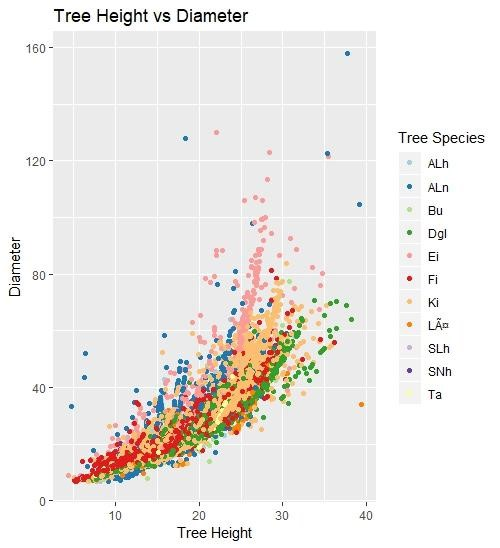
\includegraphics[scale = 0.75]{diam_vs_height.jpg}
  \caption{Relation between diameter and height. Tree species are visualized by colouring}
  \label{fig:diameter vs height}
\end{figure}

A log transformation is imposed on the response diameter (see Figure \ref{fig:log transformation diam vs height}). The log
transformation reduces the skewness of the data, while keeping a potential linear dependency. The diameter is
always positive and a log transformation can be applied. The relationship between height and log(diameter) has
improved regarding linearity.

\begin{figure}[H]
\centering
  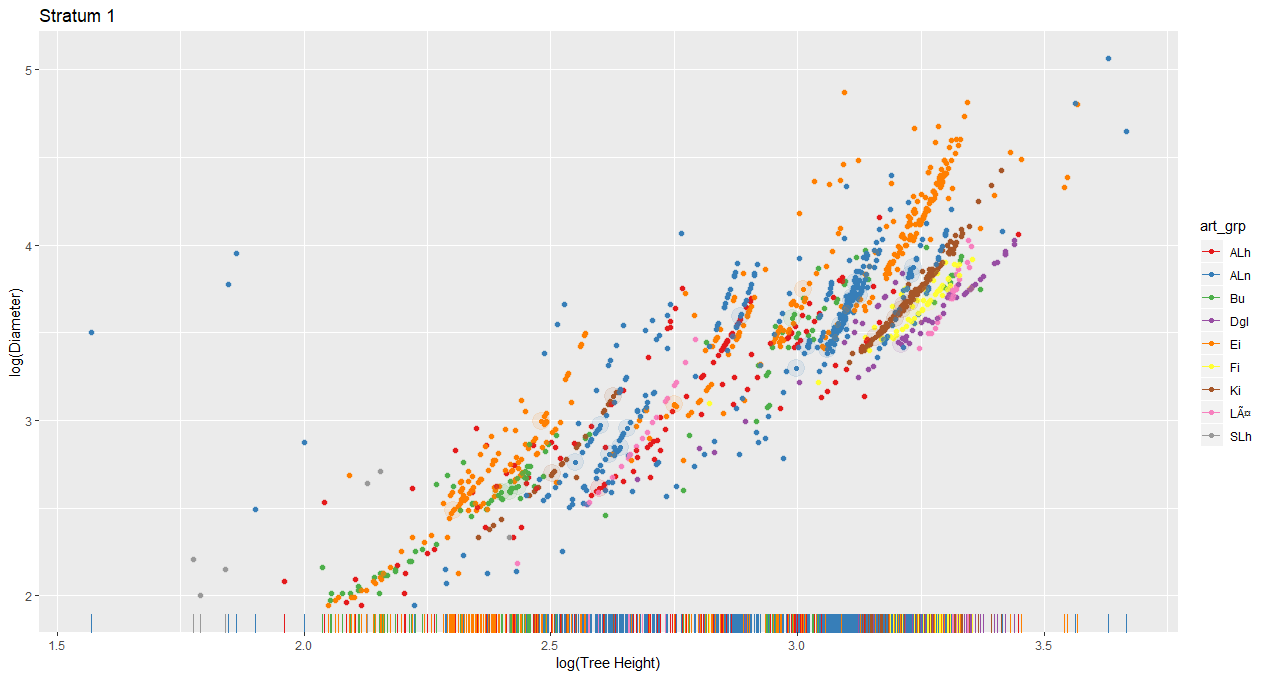
\includegraphics[scale = 0.45]{log_diam_vs_height.png}
  \caption{Scatterplot of log transformed diameter and height for Stratum 1.}
  \label{fig:log transformation diam vs height}
\end{figure}


